\documentclass{beamer}
\mode<presentation>
\usepackage[italian]{babel}
\usepackage[utf8]{inputenc}
\usepackage{fancyvrb,newverbs}
\usepackage{booktabs}
\usepackage{algpseudocode,algorithm}
\usepackage{xcolor}
\usepackage[binary-units]{siunitx}
\usepackage{hhline,colortbl,multirow}
\usepackage{listings}
\usetheme{metropolis}           % Use metropolis theme

\usepackage{mathtools} 
\DeclarePairedDelimiter{\ceil}{\lceil}{\rceil}

\DeclareSIUnit\req{req}
\definecolor{Maroon}{cmyk}{0, 0.87, 0.68, 0.32}
\definecolor{dgreen}{rgb}{0.,0.6,0.}

% Definisce comandi \cverb e \ctexttt per codice inline formattato con 
% un leggero fondale grigio che lo evidenzia rispetto al testo normale.
\definecolor{cverbbg}{gray}{0.95}
%\colorlet{cverbbg}{LemonChiffon1}
\newcommand{\ctexttt}[1]{\colorbox{cverbbg}{\texttt{#1}}}
\newverbcommand{\cverb}
  {\setbox\verbbox\hbox\bgroup}
  {\egroup\colorbox{cverbbg}{\box\verbbox}}
\newcommand{\mystrut}{\vrule height6.0pt depth0pt width0pt}
\newverbcommand{\cverbfull} % full height box
  {\setbox\verbbox\hbox\bgroup}
  {\egroup\colorbox{cverbbg}{\box\verbbox\mystrut}}

% Colore di sfondo (definito da xcolor, copiato qui), usato
% per lo sfondo dei listati.
\definecolor{LemonChiffon1}{RGB}{255,250,205}

% Configurazione estetica di default dei listati
\lstset{
  stepnumber=1,
  frame=tb,
  framexleftmargin=0.5em,
  framexrightmargin=0.5em,
  aboveskip=3mm,
  belowskip=3mm,
  columns=flexible,
  stringstyle=\color{red},
  basicstyle=\ttfamily\footnotesize,
  tabsize=4,
  backgroundcolor=\color{LemonChiffon1},
}

% Definzione della colorazione per le sessioni Redis
\lstdefinelanguage{Redis}{
  morekeywords={
    OK, QUEUED,
    SET, GET, DEL, STRLEN, INCR, INCRBY, DECRBY, GETRANGE, APPEND,
    RPUSH, LINDEX, LPOP, LLEN, LINSERT, LRANGE, AFTER,
    HSET, HMSET, HLEN, HGET, HGETALL, HKEYS, HVALS, HEXISTS,
    SADD, SISMEMBER, SREM, SCARD, SDIFF, SINTER,
    ZADD, ZCARD, ZSCORE, ZRANGE, ZREVRANGE, ZRANGEBYSCORE, ZINCRBY, ZREM,
    PFADD, PFCOUNT, 
    SCRIPT, LOAD,
    EVALSHA,
    WATCH, MULTI, EXEC,
    EXPIREAT, TTL, PTTL, PEXPIRE,
    BFADD, BFCOUNT, BFEXIST, ELEMENTS, ERROR, BFDEBUG, STATUS, FILTER,
  }, 
  sensitive=true,
  moredelim=[s][\color{Maroon}\bfseries]{127}{>},
  morestring=[b]", 
}

\lstnewenvironment{redis}[1][]
  {\lstset{
    language=Redis,
    escapechar=|,
    #1
  }}{}

\lstdefinestyle{redis}{
    language=Redis,
    escapechar=|,
}

\lstdefinestyle{csource}{
    language=C,
    includerangemarker=false,
    escapeinside={/*@}{@*/},
    numbers=left,
}


\title{Aggiunta dei filtri di Bloom al database NoSQL Redis}
\date{\today}
\author{Giovanni Bajo}
\institute{Università agli Studi di Firenze - Dipartimento di Informatica}

\begin{document}
 	\maketitle

 	\begin{frame}
	  	\frametitle{Indice}
		\tableofcontents
	\end{frame}













	\section{Redis: un database NoSQL orientato alle strutture dati}

	\begin{frame}{Redis: cos'è}
	  	\begin{block}{Un database NoSQL}
	    I database NoSQL coprono un ampio spettro di software completamente eterogenei tra loro, adatti a scopi e situazioni diverse, con l'unico tratto comune di non utilizzare il modello relazionale.
	  	\end{block}

	  	\begin{block}{Orientato alle strutture dati}
		Redis implementa un array associativo (tramite tabella hash) in cui le
chiavi sono stringhe, e i valori associati sono strutture dati: liste, insiemi, tabelle hash,
insiemi ordinati, HyperLogLog.
	  	\end{block}	

	  	\begin{block}{Veloce perché senza I/O}
L'intero dataset di chiavi e valori viene memorizzato primariamente in RAM e solo
successivamente serializzato su disco con alcune politiche di persistenza
configurabili.
		\end{block}
	\end{frame}

	\begin{frame}{Redis: dove viene usato}
	  	\begin{block}{Casi d'uso}
	  	\begin{itemize}
	  		\item Cache distribuita e intelligente
	  		\item Sistema di code di messaggi
	  		\item Distribuzione di informazioni (pub/sub)
	  	\end{itemize}
	  	\end{block}

	  	\begin{block}{Ampia adozione nell'industria}
	  	Twitter, GitHub, Instagram, AirBnb, Pinterest, Snapchat, StackOverflow, Flickr, \dots
	  	\end{block}
	\end{frame}

	\begin{frame}[fragile]{Redis: performance}
	\begin{columns}[c]
		\begin{column}{7cm}
		\begin{table}
			\centering
			\begin{tabular}{lS[table-format=5.2,table-number-alignment=center]}
				\toprule
				\rowcolor{blue!25} Nome del test & {Velocità (\SI{}{\req\per\sec})} \\
				\midrule
				\cverb|PING_INLINE| & 60132.29 \\
				\cverb|PING_BULK| & 62344.14 \\
				\midrule
				\cverb|SET| & 59988.00 \\
				\cverb|GET| & 61538.46 \\
				\cverb|INCR| & 61652.28 \\
				\cverb|LPUSH| & 61312.08 \\
				\cverb|RPUSH| & 61500.61 \\
				\midrule
				\cverb|LRANGE_100| & 20321.07 \\
				\cverb|LRANGE_300| & 8129.42 \\
				\cverb|LRANGE_500| & 6503.64 \\
				\midrule
				\cverb|MSET| (10 keys) & 32216.49 \\
				\bottomrule
			\end{tabular}
		\end{table}
		\end{column}
		\begin{column}{3cm}
		Velocità di Redis su Intel I7-6567U \SI{3.3}{\giga\hertz} con 50 client paralleli
		\end{column}
		\end{columns}
	\end{frame}









	\section{I filtri di Bloom}

	\begin{frame}{Filtri di Bloom: cosa sono}
	  	\begin{block}{Struttura dati probabilistica}
			Un filtro di Bloom è una rappresentazione probabilistica di un insieme di elementi.
			L'informazione nella tabella hash viene in parte scartata, rendendo comunque possibili alcune operazioni.
	  	\end{block}

	  	\begin{block}{Test di appartenenza}
	  		il test di appartenenza restituisce un esito probabilistico: per alcuni valori, il test ha successo anche se non effettivamente presenti
	  		(\emph{falsi positivi}).
	  	\end{block}

	  	\begin{block}{Controllo probabilità di errore}
			Il margine di errore può essere
			controllato tramite alcuni parametri, che vengono stabiliti al momento della creazione del filtro
			stesso.
			\end{block}
	\end{frame}


	\begin{frame}{Filtri di Bloom: inserimento}

		\begin{block}{Inserimento $A$: $h_1(A)=1, h_2(A)=8$}
		\begin{tabular}{*{11}{|c}|}
			\multicolumn{1}{c}{0} & \multicolumn{1}{c}{1} & \multicolumn{1}{c}{2} &
			\multicolumn{1}{c}{3} & \multicolumn{1}{c}{4} & \multicolumn{1}{c}{5} &
			\multicolumn{1}{c}{6} & \multicolumn{1}{c}{7} & \multicolumn{1}{c}{8} &
			\multicolumn{1}{c}{9} & \multicolumn{1}{c}{10} \\
		\hline
		0 & \cellcolor{blue!25}1 & 0 & 0 & 0 & 0 & 0 & 0 & \cellcolor{blue!25}1 & 0 & 0 \\
		\hline
		\end{tabular}
		\end{block}

		\vfill
		\hrule
		\vfill

		\begin{block}{Inserimento $B$: $h_1(B)=10, h_2(B)=4$}
			\begin{tabular}{*{11}{|c}|}
			\multicolumn{1}{c}{0} & \multicolumn{1}{c}{1} & \multicolumn{1}{c}{2} &
			\multicolumn{1}{c}{3} & \multicolumn{1}{c}{4} & \multicolumn{1}{c}{5} &
			\multicolumn{1}{c}{6} & \multicolumn{1}{c}{7} & \multicolumn{1}{c}{8} &
			\multicolumn{1}{c}{9} & \multicolumn{1}{c}{10} \\
		\hline
		0 & 1 & 0 & 0 & \cellcolor{blue!25}1 & 0 & 0 & 0 & 1 & 0 & \cellcolor{blue!25}1 \\
		\hline
		\end{tabular}
		\end{block}

		\vfill
		\hrule
		\vfill

		\begin{block}{Inserimento $C$: $h_1(C)=7, h_2(C)=1$}
		\begin{tabular}{*{11}{|c}|}
			\multicolumn{1}{c}{0} & \multicolumn{1}{c}{1} & \multicolumn{1}{c}{2} &
			\multicolumn{1}{c}{3} & \multicolumn{1}{c}{4} & \multicolumn{1}{c}{5} &
			\multicolumn{1}{c}{6} & \multicolumn{1}{c}{7} & \multicolumn{1}{c}{8} &
			\multicolumn{1}{c}{9} & \multicolumn{1}{c}{10} \\
		\hline
		0 & \cellcolor{blue!5}1 & 0 & 0 & 1 & 0 & 0 & \cellcolor{blue!25}1 & 1 & 0 & 1 \\
		\hline
		\end{tabular}
		\end{block}

	\end{frame}

	\begin{frame}{Filtri di Bloom: test di appartenenza}
		
		\begin{block}{Test $B$: $h_1(B)=10, h_2(B)=4$ \hfill \textbf{\textcolor{dgreen}{PRESENTE}}}
		  \begin{tabular}{*{11}{|c}|}
		  	\multicolumn{1}{c}{0} & \multicolumn{1}{c}{1} & \multicolumn{1}{c}{2} &
		  	\multicolumn{1}{c}{3} & \multicolumn{1}{c}{4} & \multicolumn{1}{c}{5} &
		  	\multicolumn{1}{c}{6} & \multicolumn{1}{c}{7} & \multicolumn{1}{c}{8} &
		  	\multicolumn{1}{c}{9} & \multicolumn{1}{c}{10} \\
		    \hline
		    0 & 1 & 0 & 0 & \cellcolor{green!35}1 & 0 & 0 & 1 & 1 & 0 & \cellcolor{green!35}1 \\
		    \hline
		  \end{tabular}
		\end{block}

		\vfill
		\hrule
		\vfill

		\begin{block}{Test $E$: $h_1(E)=0, h_2(E)=7$ \hfill \textbf{\textcolor{dgreen}{ASSENTE}}}
		  \begin{tabular}{*{11}{|c}|}
		  	\multicolumn{1}{c}{0} & \multicolumn{1}{c}{1} & \multicolumn{1}{c}{2} &
		  	\multicolumn{1}{c}{3} & \multicolumn{1}{c}{4} & \multicolumn{1}{c}{5} &
		  	\multicolumn{1}{c}{6} & \multicolumn{1}{c}{7} & \multicolumn{1}{c}{8} &
		  	\multicolumn{1}{c}{9} & \multicolumn{1}{c}{10} \\
		    \hline
		    \cellcolor{red!35}0 & 1 & 0 & 0 & 1 & 0 & 0 & \cellcolor{green!35}1 & 1 & 0 & 1 \\
		    \hline
		  \end{tabular}
		\end{block}

		\vfill
		\hrule
		\vfill

		\begin{block}{Test $F$: $h_1(F)=4, h_2(F)=8$ \hfill \textbf{\textcolor{red}{FALSO POSITIVO}}}
		  \begin{tabular}{*{11}{|c}|}
		  	\multicolumn{1}{c}{0} & \multicolumn{1}{c}{1} & \multicolumn{1}{c}{2} &
		  	\multicolumn{1}{c}{3} & \multicolumn{1}{c}{4} & \multicolumn{1}{c}{5} &
		  	\multicolumn{1}{c}{6} & \multicolumn{1}{c}{7} & \multicolumn{1}{c}{8} &
		  	\multicolumn{1}{c}{9} & \multicolumn{1}{c}{10} \\
		    \hline
		    0 & 1 & 0 & 0 & \cellcolor{green!35}1 & 0 & 0 & 1 & \cellcolor{green!35}1 & 0 & 1 \\
		    \hline
		  \end{tabular}
		\end{block}

	\end{frame}


	\begin{frame}{Filtri di Bloom: utilizzo}

	  	\begin{block}{Pubblicati nel 1970}
	  	Primo utilizzo: sistema di sillabazione del testo in lingua inglese,
	  	per gestione eccezioni alle regole base.
	  	\end{block}

	  	\begin{block}{Alcuni casi d'uso odierni}
	  	\begin{itemize}
	  		\item Sincronizzazione di cache distribuite (CDN)
	  		\item Controllo anti-phishing nei browser
	  		\item Routing nelle reti P2P
	  	\end{itemize}
	  	\end{block}

	\end{frame}


	\begin{frame}[fragile]{Filtri di Bloom: parametri}
	\begin{columns}[c]
		\begin{column}{6cm}
			\begin{tabular}{cp{5cm}}
				\toprule
				$M$ & Dimensione in bit dell'array. \\
				$K$ & Numero delle funzioni di hash. \\
				$N$ & Numero di elementi presenti nel filtro. \\
				$P$ & Probabilità di un falso positivo. \\
				\bottomrule
			\end{tabular}
		\end{column}

		\begin{column}{5cm}
		$$ N \approx \ceil*{M\frac{\ln(0.5)^2}{|\ln(P)|}} $$
		$$ P \approx 0.6185^{\frac{M}{N}} $$
		$$ K = \ceil*{-\log_2{P}} $$
		\end{column}
	\end{columns}
	\end{frame}

	\begin{frame}[fragile]{Filtri di Bloom: ottimizzazione filtro 64 MiB}
			\begin{figure}
				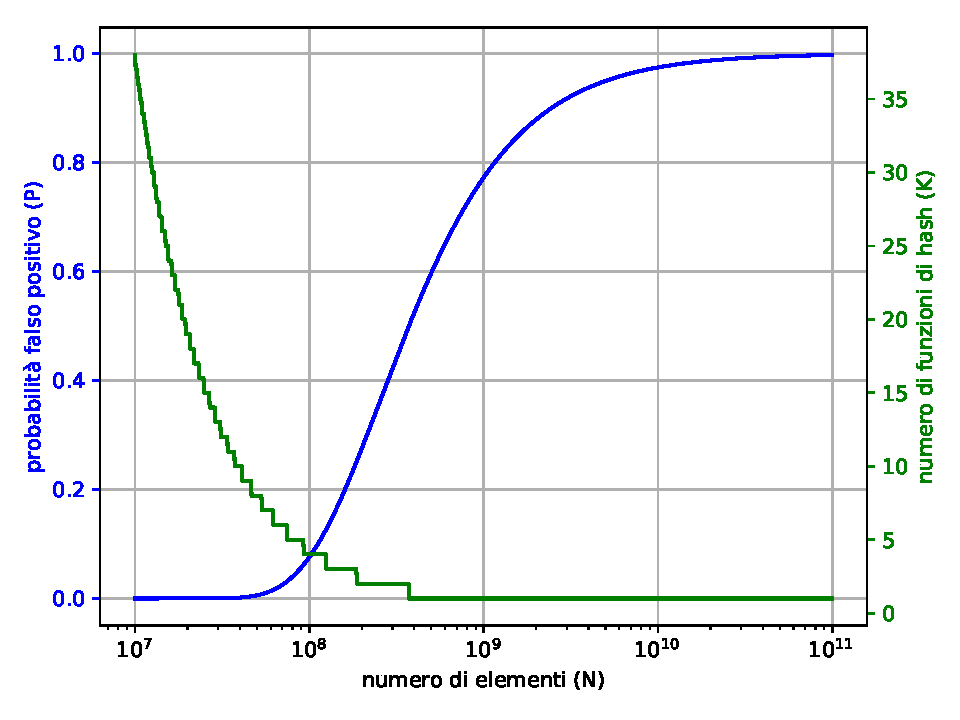
\includegraphics[width=\textwidth]{img/bloom_parms_2}
			\end{figure}
	\end{frame}










	\section{Aggiunta dei filtri di Bloom a Redis}

	\begin{frame}{Contesto della modifica}
	  	\begin{block}{Redis è scritto in C}
	  	120K linee di codice, con copertura test automatizzati in Lua.
	  	Necessità di capire la struttura della base di codice e trovare
	  	i punti di innesto.
	  	\end{block}

	  	\begin{block}{Scrittura di codice allineato agli standard}
	  	Obiettivo concreto di contribuzione e integrazione nella base di codice. Trattandosi di un progetto open source, ho stabilito una comunicazione con il maintainer del progetto.
	  	\end{block}

	  	\begin{block}{Approccio alle performance critico}
	  	Algoritmi scritti tenendo conto dei tempi di esecuzione di
	  	ciascuna singola istruzione, strutturate dati ottimizzate
	  	anche a livello di accesso di cache.
	  	\end{block}
	\end{frame}

	\begin{frame}{Focus: filtri scalabili di Bloom}

	  	\begin{block}{Necessità di scalabilità infinita}
	  	Nessuna struttura dati di Redis è preallocata staticamente,
	  	e può crescere senza limiti, fino ad esaurimento della RAM.
	  	\end{block}

	  	\begin{block}{Utilizzo dei filtri scalabili di Bloom}
	  	Variante che concatena più filtri di Bloom con dimensione
	  	esponenzialmente crescente, mantenendo la probabilità 
	  	richiesta a livello asintotico.
	  	\end{block}

	\end{frame}

	\begin{frame}[fragile]{Focus: algoritmo di hash doppio}
		\begin{algorithmic}[1]
		\Procedure{EnhancedDoubleHash}{$x$, $h_a$, $h_b$}
			\State $a \gets h_a(x)$
			\State $b \gets h_b(x)$
			\State $h(1) \gets a \bmod M$
			\For {$i=2$ \textbf{to} $K$}
				\State $a \gets a+b$
				\State $b \gets b+i$
				\State $h(i) \gets a \bmod M$
			\EndFor
			\State \Return $h$
		\EndProcedure
		\end{algorithmic}
	\end{frame}

	\begin{frame}[fragile]{Test di appartenenza}
		\begin{lstlisting}[language=C]
		int bloomFilterExist(filter *flt, uint64_t hash) {
		    uint32_t a = (uint32_t)hash;
		    uint32_t b = (uint32_t)(hash>>32);

		    for (unsigned int i=0;i<flt->k;i++) {
		        uint64_t index = a;
		        a += b; b += i;
		        index = (index * flt->s) >> 32;

		        if (~(flt->parts[i][index>>3] >> (index & 7)) & 1)
		            return 0;
		    }
		    return 1;
		}
		\end{lstlisting}
	\end{frame}

	\begin{frame}{Risultati e sviluppi futuri}

		\begin{block}{Funzionalità completata}
		L'obiettivo del lavoro è stato raggiunto tramite
		un lavoro di design volto a cercare di rispettare tutte le convenzioni usate dai comandi esistenti, lo stile del sorgente scritto, e  l'architettura interna del codice.
		\end{block}

		\begin{block}{Implementazione curata}
		L'implementazione è stata curata dal punto di vista delle performance e dell'uso della memoria, I test automatici scritti, di cui alcuni molto ampi, confermano la correttezza della implementazione.
		\end{block}

		\begin{block}{Fusione alla base di codice principale}
		Il codice scritto rispecchia dunque tutti gli standard di qualità di Redis ed è potenzialmente integrabile nella base di codice fin da subito.
		\end{block}

	\end{frame}

\end{document}
